\documentclass[./main.tex]{subfiles}


\begin{document}

\newcommand{\ob}{\textit{1B} }
\newcommand{\fb}{$\forall$\textit{1B} }
\newcommand{\cb}{\textit{CB} }
\newcommand{\dbb}{\textit{DB} }

\chapter{Implementazione di procedure di decisione per frammenti Binding in Vampire}
In questo capitolo verrà descritto in che modo è stato implementato l'algoritmo di decisione per frammenti Binding 
introdotto nel capitolo \ref{chap:binding} utilizzando gli strumenti 
e le funzionalità descritte nel capitolo \ref{chap:vampire} offerte da Vampire.
Per ragioni di integrazione e manutenibilità del codice,
si è deciso di limitare le modifiche alle funzioni e al Kernel di Vampire al minimo indispensabile, 
privilegiando l'impiego di componenti e funzionalità preesistenti. 
Questa decisione, tuttavia, ha comportato alcune complessità nell'implementazione, 
e questo è evidente nella sezione \ref{sec:preprocessing}. 
Non tutti gli algoritmi standard di Vampire sono direttamente applicabili alle formule dei frammenti binding. 
Di conseguenza, anziché apportare modifiche dirette alle funzioni del kernel, 
si è optato per la creazione di strutture ausiliarie al fine di garantire la coerenza con la formula originale,
sebbene ciò possa incidere sull'efficienza del sistema. 
Ad esempio si può notare che la procedura di preprocessing genera un elevato numero di nuovi letterali; 
tuttavia, mediante la modifica delle funzioni del kernel, sarebbe possibile ridurlo anche del 50\%.
Nonostante ciò, l'obiettivo primario di questo studio rimane confrontare l'approccio adottato con un approccio
general-purpose basato su Resolution e GivenClause Architecture. 
È importante sottolineare che la fase di preprocessing, che è il componente meno ottimizzato,
è esclusa dalla misurazione, 
pertanto non rappresenta un ostacolo significativo nel confronto tra i due approcci.



\section{Preprocessing} \label{sec:preprocessing}

\begin{figure}[H]
    \centering
    \scalebox{0.55}{
        \includesvg{images/4_progettazione/Preprocess.svg}
    }
    \caption{Struttura del Preprocessing}
    \label{fig:preprocessing}
\end{figure}

In questa sezione verrà descritto l'algoritmo di preprocessing utilizzato per trasformare una formula in input
del frammento \ob o \cb in una struttura trattabile dall'algoritmo di decisione.
Per utilizzare il SatSolver di Vampire per la ricerca degli implicanti è necessario clausificare la formula.
Inoltre per evitare un esplosione esponenziale di formule causate dalle forme NNF e CNF è necessario utilizzare tecniche di naming.
Qui sorgono i primi problemi visto che ne la clausificazione ne il naming sono processi conservativi rispetto ai frammenti.
Ad esempio la semplice formula del frammento \ob $\forall x_1 (p_1(x_1)) \lor p_2$ clausificata diventa  $\{\{p_1(x_1), p_2\}\}$ che fa parte del frammento \dbb.
L'approccio utilizzato è stato quello di creare una nuova formula ground che rappresenta la struttura booleana esterna della formula originale,
applicare le funzioni standard di preprocessing
e mantenere una serie di strutture per risalire ai componenti originali.
Per questo scopo viene introdotto un nuovo insieme di simboli di predicato $\Sigma_b = \{b_1, b_2, ...\}$.
I predicati di $\Sigma_b$ con arietà 0 saranno chiamati \textit{booleanBinding} e saranno associati ad una formula del frammento \ob o \cb.
I predicati di $\Sigma_b$ con arietà $n > 0$ saranno chiamati \textit{literalBindign} e fungeranno da rappresentati dei $\tau$-Binding delle formule \ob.
Il preprocessing seguirà pressochè questa struttura:

\begin{enumerate}
    \item Rettificazione
    \item Trasformazione in ENNF
    \item Creazione della formula booleana esterna (FBE) e associazione dei booleanBinding
    \item Naming della FBE
    \item Trasformazione in NNF della FBE
    \item Creazione dei literalBinding e Sat-Clausificazione delle formule associate ai booleanBinding
    \item Creazione delle Sat-Clausole della FBE
\end{enumerate}

La rettificazione e la trasformazione in ENNF sono processi conservativi rispetto ai frammenti e quindi verranno applicate 
direttamente le funzioni standard di Vampire.
La creazione della FBE e l'associazione dei booleanBinding avviene tramite l'algoritmo \ref{alg:topBooleanFormula}.

\begin{algorithm}[H] \label{alg:topBooleanFormula}
    \caption{Top Boolean Formula}
    \KwSty{Firma:}{ topBooleanFormula($\varphi$)}\\
    \KwIn{$\varphi$ una formula rettificata}
    \KwOut{Una formula ground}
    \KwSty{GlobalData: }{ bindingFormulas una mappa da booleanBinding a formula}
\Switch{$\varphi$}{

\Case{Literal l}{
    \Return new AtomicFormula(l)\;
}
\Case{A$[\land, \lor]$B}{
    \Return new JunctionFormula(topBooleanFormula(A), connective of $\varphi$, topBooleanFormula(B))\;
}
\Case{$\lnot$A}{
    \Return new NegatedFormula(topBooleanFormula(A))\;
}
\Case{$[\forall, \exists]$A}{
    $b = newBooleanBinding()$\;
    $bindingFormulas[b] := \varphi$\;
    \Return new AtomicFormula(b)\;
}

\Case{A$[\leftrightarrow, \rightarrow, \oplus]$B}{
    \Return new BinaryFormula(A, connective of $\varphi$, B)\;
}
}
\end{algorithm}

L'algoritmo prende in input una formula rettificata e restituisce una formula ground sostituendo le sottoformule quantificate con 
un nuovo booleanBinding aggiungendo la sottoformula originale alla mappa bindingFormulas.
Da adesso in poi qualunque modifica fatta alla FBE preserverà l'appartenenza al frammento originale.
Gli step successivi sono quindi applicare le funzioni standard di Vampire per il naming e la trasformazione in NNF.
La trasformazione in NNF potrebbe portare alla negazione di qualche booleanBinding
e va quindi aggiunta alla mappa bindingFormulas la formula negata associata.

\ForEach{$l \in literals(\varphi)$}{
    \If{$\lnot$l.polarity()}{
        \textbf{continue}
    } 
    $positiveFormula := bindingFormulas[positiveLiteral(l)]$\; \\
    $bindingFormulas[l] := new NegatedFormula(positiveFormula)$\;
}

A questo punto inizia il processo di SatClausificazione delle formule interne (quelle associate ai booleanBinding).
Ogni letterale ground che non è un booleanBinding viene trasformato in una 
SatClausola di lunghezza 1 composta dal solo satLetterale associato al letterale.

\ForEach{$l \in literals(\varphi)$}{
    \If{$l$ is not a booleanBinding}{
        $bindingClauses[l] := new SatClause\{toSat(l)\}$\;
    }
}

Per essere clausificate le formule della mappa bindingFormulas vanno trasformate in NNF, Skolemizzate.
Anche in questo caso vengono utilizzate le funzioni standard di Vampire. 
Ogni booleanBinding è associato ad una formula del frammento ConjunctiveBinding,
per questo dopo la skolemizzazione il quantificatore universale viene distribuito sull'and per ottenere le sottoformule del frammento OneBinding.
Per ogni sottoformula OneBinding viene creato un nuovo LiteralBinding in rappresentaza della sottoformula.
Il nuovo letterale avrà gli stessi termini del letterale più a sinistra della sottoformula (che sono gli stessi di tutti i letterali della sottoformula).
Successivamente la formula viene SatClausificata. 
Si aggiunge alla mappa satClauses la coppia composta dal nuovo LiteralBinding e le satClausole della sottoformula.
Alla mappa literalToBooleanBindings viene aggiunta la coppia composta dal nuovo LiteralBinding e il booleanBinding associato mentre alla mappa
booleanBindingToLiteral viene aggiunta la coppia composta dal booleanBinding e la lista dei LiteralBinding che rappresentano le sottoformule della formula originale.  


\While{bindingFormulas $\neq \emptyset$}{
    $(booleanBinding, formula) := bindingFormulas.pop()$\;\\
    $formula := nnf(formula)$\;\\
    $formula := skolemize(formula)$\;\\
    $toDo := \emptyset$\;\\

    \If{formula is ConjunctiveBinding}{
        $formula := distributeForAll(formula)$\;\\
        "Add each subformula to the todo list"\;
    } \Else{
        toDo.add(formula)\;
    }

    $literalBindings := \emptyset$\;\\
    \While{todo $\neq \emptyset$}{
        $subformula := todo.pop()$\;\\
        $literalBinding := newLiteralBinding(subformula.mostLeftLiteral())$\;\\
        $clauses := SatClausifyBindingFormula(subFormula)$\;\\

        $satClauses[literalBinding] := clauses$\;\\
        $literalToBooleanBindings[literalBinding] := booleanBinding$\;\\
        $literalBindings.add(literalBinding)$\;\\
    }
    $booleanBindingToLiteral[booleanBinding] := literalBindings$\;
}

La funzione SatClausifyBindingFormula è una funzione che prende in input una formula
la clausifica e converte tutte le clausole in SatClausole in modo che ogni satLetterale ha lo stesso indice del funtore del predicato associato.
Questo è differente da quello che viene fatto dalla classe Sat2Fo che associa ogni puntatore a letterale ad un nuovo SatLetterale con un nuovo indice arbitrario.
L'ultimo step è la SatClausificazione della FBE che avviene tramite le funzioni standard di Vampire della classe Sat2Fo.
È importante ricordare che i satLetterali delle formule interne sono diversi dai satLetterali della FBE nonostante possano avere
lo stesso indice.

Si prenda ad esempio la formula del frammento \cb:

$$ (\forall x_1, x_2 ((p_1(x_1) \lor p_2(x_1)) \land p_2(f_1(x_2))) 
\land  \forall x_1 (p_3(x_1) \rightarrow p1(x_1)))  
\lor (\forall x_1(p_2(x_1)) \rightarrow p_4)
$$

Il primo passo di preprocessing prevede la rettificazione e la trasformazione in ENNF.
La formula è già rettificata mentre la trasformazione in ENNF porta all'eliminazione del $\rightarrow$:

$$ (\forall x_1, x_2 ((p_1(x_1) \lor p_2(x_1)) \land p_2(f_1(x_2))) 
\land  \forall x_1 (\lnot p_3(x_1) \lor p1(x_1)))  
\lor (\forall x_1(p_2(x_1)) \leftrightarrow p_4)
$$

La creazione della FBE porta alla generazione di un booleanBinding per ogni sottoformula quantificata:

$$ (b_1 
\land  b_2)  
\lor (b_3 \leftrightarrow p_4)
$$

La mappa bindingFormulas contiene le seguenti coppie:

\begin{itemize}
    \item [$b_1$] $\rightarrow \forall x_1, x_2 ((p_1(x_1) \lor p_2(x_1)) \land p_2(f_1(x_2))) $
    \item [$b_2$] $\rightarrow \forall x_1 (\lnot p_3(x_1) \lor p1(x_1))$
    \item [$b_3$] $\rightarrow \forall x_1(p_2(x_1))$
\end{itemize}

La formula ottenuta è troppo piccola per poter applicare il namig
quindi si procede direttamente con la trasformazione in NNF:

$$ (b_1 
\land  b_2)  
\lor ((\lnot b_3 \lor p_4) \land (b_3 \lor \lnot p_4))
$$

Durante il processo di NNF il booleanBinding $b_3$ è stato negato e quindi va aggiunto alla mappa bindingFormulas:

\begin{itemize}
    \item [$\lnot b_3$] $\rightarrow \exists x_1(\lnot p_2(x_1))$
\end{itemize}

A questo punto vengono trasformate in NNF e Skolemizzate le formule associate ai booleanBinding,
vengono poi creati i literalBindings e le SatClausole delle formule interne.
Il booleanBinding $b_1$ è associato ad una formula \cb quindi 
viene distribuito il quantificatore universale sull'and e creati due literalBindings.
La skolemizzazione della formula associata a $\lnot b_3$ porta alla formula::
\begin{itemize}
    \item [$\lnot b_3$] $\rightarrow \lnot p_2(sk_1)$
\end{itemize}
Vengono create così le mappe booleanBindingToLiteral e la sua inversa literalToBooleanBindings:

\begin{table}[H]
    \centering
    \begin{tabular}{|c|c|}
        \hline
        \textbf{booleanBindingToLiteral} & \textbf{literalToBooleanBindings} \\
        \hline
        $b_1 \rightarrow \{b_4(x_1), b_5(f_1(x_1))\}$ & $b_4(x_1) \rightarrow b_1$\\
        $b_2 \rightarrow \{b_6(x_1)\}$ & $b_5(f_1(x_1)) \rightarrow b_1$ \\
        $b_3 \rightarrow \{b_7(x_1)\}$ & $b_6(x_1) \rightarrow b_2$ \\
        $\lnot b_3 \rightarrow \{b_8(sk_1)\}$ & $b_7(x_1) \rightarrow b_3$ \\
        & $b_8(sk_1) \rightarrow \lnot b_3$ \\
        \hline
    \end{tabular}
\end{table}

Le formule associate ai literalBindings vengono clausificate:

\begin{itemize}
    \item $\forall x_1, x_2 ((p_1(x_1) \lor p_2(x_1))) \rightarrow \{\{(p_1(x_1), p_2(x_1))\}\}$
    \item $\forall x_1, x_2 (p_2(f_1(x_2))) \rightarrow \{\{p_2(f_1(x_2))\}\}$
    \item $\forall x_1 (\lnot p_3(x_1) \lor p1(x_1)) \rightarrow \{\{\lnot p_3(x_1), p1(x_1)\}\}$
    \item $\forall x_1(p_2(x_1)) \rightarrow \{\{p_2(x_1)\}\}$
    \item $\lnot p_2(sk_1) \rightarrow \{\{\lnot p_2(sk_1)\}\}$
\end{itemize}

E successivamente SatClausificate e associate ai literalBindings:
\begin{itemize}
    \item $b_4(x_1) \rightarrow \{\{s_1, s_2\}\}$
    \item $b_5(f_1(x_1)) \rightarrow \{\{s_2\}\}$
    \item $b_6(x_1) \rightarrow \{\{\lnot s_3, s_1\}\}$
    \item $b_7(x_1) \rightarrow \{\{s_2\}\}$
    \item $b_8(sk_1) \rightarrow \{\{\lnot s_2\}\}$
\end{itemize}

Gli ultimi due step sono la clausificazione della FBE:
$$ \{\{b_1, \lnot b_3, p_4\}, \{b_2, \lnot b_3, p_4\}, \{b_1, b_3, \lnot p_4\}, \{b_2,  b_3, \lnot p_4\}\} $$
E la SatClausificazione tramite sat2Fo:
$$ \{\{s_1, \lnot s_2, s_3\}, \{s_4, \lnot s_2, s_3\}, \{s_1, s_2, \lnot s_3\}, \{s_4,  s_2, \lnot s_3\}\} $$
Che crea internamente una hashMap bidirezionale che associa ogni satletterale ad un letterale:
\begin{multicols}{2}
\begin{itemize}
    \item $s_1 \leftrightarrow b_1$
    \item $s_2 \leftrightarrow \lnot b_3$
    \item $s_3 \leftrightarrow p_4$
    \item $s_4 \leftrightarrow b_2$
\end{itemize} 
\end{multicols}



\section{Procedura di Decisione} \label{sec:decisione}
\begin{figure}[H]
    \centering
    \scalebox{0.55}{
        \includesvg{images/4_progettazione/OneBindingAlgorithm.svg}
    }
    \caption{Struttura dell'algoritmo di decisione}
    \label{fig:algoritmo_decisione}
\end{figure}

In questa sezione verrà descritta l'implementazione dell'algoritmo di decisione \ref{alg:1b}
per frammenti Binding descritto nel capitolo \ref{chap:binding}.
L'algoritmo è composto da tre parti principali: la ricerca degli implicanti,
la ricerca di tutti i sottoinsiemi unificabili e la ricerca di un assegnamento proposizionale 
che soddisfi la congiunzione della conversione booleana dei sottoinsiemi unificabili.
Da questo momento si assuma di avere una formula preprocessata con tutte le strutture ausiliarie come descritto nella sezione precedente.

La ricerca degli implicanti è la parte più facile da implementare (sat esterna). 
Data la FBE SatClausificata è sufficiente utilizzare il satSolver integrato in Vampire ed estrapolarne una assegnazione.
Dopo aver ottenuto l'insieme degli implicanti proposizionali se la sua relativa 
formula del primo ordine è insoddisfacibile allora è sufficiente creare una clausola bloccante e cercare un nuovo assegnamento.
Se non sono disponibili nuovi assegnamenti allora la formula originale è insoddisfacibile.

La ricerca di tutti i sottoinsiemi unificabili è senza dubbio la parte più complessa dell'algoritmo.
L'approccio utilizzato nell'algoritmo \ref{alg:1b} è troppo astratto e non utilizzabile nella pratica.
Anche il solo problema di iterare su tutti i sottoinsiemi di un insieme è un problema non trivale.
Vanno quindi necessariamente fatti dei tagli nello spazio di ricerca.
La prima osservazione che si può fare è che se un insieme di letterali è unificabile allora i letterali hanno tutti la stessa arietà.
È quindi possibile ordinare l'insieme di implicanti in base all'arietà e ricercare per ogni 'Gruppo di Arietà' tutti i sottoinsiemi unificabili.
Già in questo modo si riduce notevolmente lo spazio di ricerca eliminando tutti quei sottoinsiemi composti da letterali di arietà diversa.
La seconda osservazione è che dati due sottoinsiemi $U' \subseteq U$ se la congiunzione della conversione booleana dei letterali di $U$ è 
soddisfacibile allora lo sarà anche quella di $U'$. 
Questo riduce ulteriormente lo spazio di ricerca ai soli sottoinsiemi massimali unificabili.
Sfortunatamente la ricerca di tutti i sottoinsiemi massimali unificabili (Maximal Unifiable Subsets / MUS) è un problema NP-Completo così come 
il suo problema complementare cioè il problema di ricercare tutti i sottoinsiemi minimali non unificabili (minimal non unifiable subsets / mnus).
Per questo motivo è stato creato un algoritmo euristico meno restrittivo che itera almeno su tutti i sottoinsiemi massimali
non escludendo però la possibilità di trovare anche qualche sottoinsieme non massimale.

Dopo aver ottenuto un insieme di $\tau$-Binding unificabili l'algoritmo procede con la ricerca di un 
assegnamento proposizionale che soddisfi la congiunzione della conversione booleana dei sottoinsiemi unificabili (sat interna).
Anche in questo caso il problema è molto semplice. Ogni $\tau$-Binding è rappresentato da un bindingLiteral creato nella fase di preprocessing e
ogni bindingLiteral è associato ad un insieme di satClausole che rappresentano la conversione booleana citata sopra. 
Grazie a questa indicizzazione è possibile utilizzare il satSolver integrato per verificare la soddisfacibilità.


\subsubsection{Maximal Unifiable Subsets}

Per la ricerca dei mus è stato implementato un algoritmo ricorsivo che in modo incrementale costruisce un sottoinsieme di letterali unificabile.
L'algoritmo sfrutta un SubstitutionTree per la ricerca degli unificatori e una mappa S che rappresenta la funzione caratteristica 
dell'insieme soluzione. 
In particolare per ogni letterale $x$ se $S[x] = 1$ allora fa parte della soluzione, se $S[x] = 0$ allora non fa parte della soluzione
e infine se $S[x] = -1$ allora vuol dire che non fa parte della soluzione e deve essere escluso dalle ricerche future.
Prima di iniziare la ricerca va impostato l'ambiente in modo tale che il SubstitutionTree contenga tutti i letterali 
del gruppo di arietà corrente e S mappi tutti i letterali a 0. 
Viene fornita anche una funzione \textit{fun} che prende in input l'insieme soluzione e restituisce un booleano.
La funzione \ref{alg:mus_call} è la funzione che inizia la catena di chiamate ricorsive. 
% Prende in input un letterale e itera su (almeno) tutti i mus che contengono il letterale.




% La ricerca termina o quando sono finiti tutti i sottoinsiemi disponibili e in questo caso la funzione \ref{alg:mus_call} restituisce $\top$
% oppure appena la funzione \textit{fun} restituisce $\bot$ e in questo caso la funzione \ref{alg:mus_call} propaga il risultato restituendo $\bot$.


\begin{algorithm}[H] \label{alg:mus_call}
    \caption{Maximal Unifiable Subsets}
    \KwSty{Firma:}{ mus($literal$)}\\
    \KwIn{$literal$ un puntatore ad un letterale}
    \KwOut{$\top$ o $\bot$}
    \KwSty{GlobalData: }{ S una mappa da letterali a interi}

\nl \If{$S[literal] \neq 0$}{
    \Return $\top$\;
}
\nl \If{$literal$ is ground}{
    \Return $groundLiteralMus(literal)$\;
}

$S[literal] = 1$\;
$tmpToFree := \emptyset$\;
$res := mus(literal, tmpToFree)$\;
\ForEach{$i \in tmpToFree$}{
                $S[i] = -1$\;
            }
$S[literal] = -1$\;
\Return $res$\;
\end{algorithm}

Inizialmente verifica se il letterale è già stato esplorato e in quel caso restituisce $\top$.
Se il letterale è ground allora chiama la funzione \ref{alg:groundMus} che è un'ottimizzazione pensata 
per semplificare la ricerca con letterali ground.
Se il letterale non è ground allora si inizia la vera e propria ricerca dei mus.
Viene impostato il valore del letterale nella mappa S ad 1 in modo tale che faccia parte della soluzione 
e chiama la funzione \ref{alg:mus} che prende in input il letterale e un insieme di letterali.


\begin{algorithm}[H] \label{alg:mus}
    \small
    \caption{Maximal Unifiable Subsets}
    \KwSty{Firma:}{ mus($literal$, $FtoFree$)}\\
    \KwIn{$literal$ un puntatore ad un letterale, $FtoFree$ un puntatore ad una lista di letterali}
    \KwOut{$\top$ o $\bot$}
    \KwSty{GlobalData: }{ \textbf{S} una mappa da letterali a interi, \textbf{fun} una funzione da lista di letterali a bool, \textbf{tree} un SubstitutionTree}

$isMax := \top$\;
$uIt = tree.getUnifications(query: literal, retrieveSubstitutions: true)$\;
$toFree := \emptyset$\;

\While{$uIt.hasNext()$}{
    $(u, \sigma) := uIt.next()$\;
    \If{$S[u] = 0$}{
        $S[u] = 1$\;

        $l := literal^\sigma$\;
        \nl \If{$l = literal$} {
            $u' := u^\sigma$\;
            \If{$u' = u$}{
                $FtoFree := FtoFree \cup \{u\}$\;
            } \Else{
                $toFree := toFree \cup \{u\}$\;
            }
        }
        \Else{
            $isMax = \bot$\;
            $tmpToFree := \emptyset$\;
            \If{$\neg mus(l, tmpToFree)$}{
                \Return $\bot$\;
            }
            $S[u] = -1$\;
            \ForEach{$i \in tmpToFree$}{
                $S[i] = -1$\;
            }
            $toFree := toFree \cup \{u\} \cup tmpToFree$\;
        }
    }
}
\If{$isMax$}{
    \If{$\neg fun(\{x \mid S[x] =1\})$}{
        \Return $\bot$\;
    }
}
\While{$toFree \neq \emptyset$}{
    $S[toFree.pop()] = 0$\;
}
\Return $\top$\;
\end{algorithm}

La funzione comincia inizializzando la variabile $isMax$ a $\top$ che rappresenta il fatto che il sottoinsieme è massimale.
Se non vengono effettuate chiamate ricorsive allora $isMax$ non viene modificato
e viene chiamata la funzione \textit{fun} sull'insieme soluzione.
Successivamente viene chiesto al SubstitutionTree di restituire un iteratore
su tutti i letterali unificabili con il letterale in input.
Viene inizializzata una lista $toFree$ che conterrà tutti gli elementi che 
verranno bloccati su questo livello dell'albero delle chiamate ricorsive.

Per capire meglio questo aspetto dell'algoritmo si consideri un insieme di 
letterali $\{l_1, ... , l_n\}$. Un modo di ottenere tutti i mus di questo insieme,
che è anche il modo che è stato implementato,
è quello di cercare tutti i mus che contengono $l_1$, tutti i mus che contengono $l_2$ e così via.
Si supponga di aver già trovato tutti i mus che contengono $l_1$ e di 
voler cercare tutti i mus che contengono $l_2$. 
Se l'algoritmo rileva che $l_2$ è unificabile con $l_1$ tramite la sostituzione $\sigma$,
dovrebbe inserire $l_1$ nella soluzione e cercare tutti i mus
che contengono $l_2^\sigma$ e così via.
Ma si può notare che mus di questo tipo sono già stati esplorati quando 
si cercavano i mus che contenevano $l_1$.
Per questo motivo in modo da evitare di ripetere del lavoro già svolto,
alla fine della ricerca dei mus che contengono $l_1$, il letterale viene
bloccato ($S[l_1] = -1$) e viene aggiunto ad una lista $toFree$.
In generale per ogni $l_x$ vengono cercati tutti i mus che contengono $l_x$
escludendo dalla ricerca i letterali $l_y$ con $y < x$.
Una volta arrivati ad $l_n$ si liberano ($S[l_{(...)}] = 0$) tutti i letterali bloccati in $toFree$.

Tornando alla descrizione dell'algoritmo, dopo aver inizializzato la lista $toFree$
si itera su tutti i letterali che unificano con il letterale in input $literal$.
Per ogni letterale $u$ se è già contenuto nella soluzione, o è stato bloccato, si ignora,
altrimenti viene aggiunto alla soluzione.
Si calcola il letterale $l = literal^\sigma$ ottenuto applicando la sostituzione
$\sigma$ al letterale $literal$. 
Se il letterale $l$ è uguale a $literal$, cioè la sostituzione non ha 
apportato nessun cambiamento, 
allora si evita di effettuare una chiamata ricorsiva su $l$ in quanto è possibile
utilizzare lo stesso iteratore di $literal$. 
Se anche $u^\sigma$ è uguale a $u$ allora viene aggiunto alla lista $FtoFree$ passata in input.
Questo perchè $u$ ha esattamente gli stessi termini di $literal$ quindi tutti i mus che contengono $u$ contengono anche $literal$.
$u$ va quindi rimosso/bloccato/sbloccato dalla soluzione esattamente quando viene rimosso/bloccato/sbloccato il letterale
con cui è stata fatta l'unificazione al livello superiore che ha poi generato $literal$.
In caso contrario viene aggiunto alla lista $toFree$ per essere rimosso alla fine dell'esecuzione del livello corrente.

Se il letterale $l$ è diverso da $literal$ non è detto che la soluzione corrente sia massimale,
quindi si imposta $isMax$ a $\bot$ e viene effettuata una chiamata ricorsiva dando come parametri $l$
e una lista temporanea $tmpToFree$. 
Nel caso la chiamata ricorsiva restituisca $\bot$ allora la funzione propaga il risultato negativo restituendo $\bot$.
Dopo la chiamata ricorsiva il letterale $u$ viene rimosso dalla soluzione e bloccato per 
questo livello della ricorsione. Viene poi aggiunto alla lista $toFree$ per essere sbloccato 
alla fine dell'esecuzione del livello corrente.
Vengono anche bloccati tutti i letterali restituiti dalla chiamata ricorsiva tramite la lista $tmpToFree$ e aggiunti a $toFree$
per essere sbloccati alla fine dell'esecuzione del livello corrente.

Alla fine dell'iterazione sui letterali unificabili se $isMax$ è $\top$ 
allora si compone la soluzione e viene chiamata la funzione \textit{fun}.
Se \textit{fun} restituisce $\bot$ allora si restituisce $\bot$.
Altrimenti si liberano i letterali della lista $toFree$ e si restituisce $\top$.


\begin{algorithm}[H] \label{alg:groundMus}
    \caption{Maximal Unifiable Subsets Ground}
    \KwSty{Firma:}{ groundMus($literal$)}\\
    \KwIn{$literal$ un puntatore ad un letterale ground}
    \KwOut{$\top$ o $\bot$}
    \KwSty{GlobalData: }{ \textbf{S} una mappa da letterali a interi, \textbf{fun} una funzione da lista di letterali a bool, \textbf{tree} un SubstitutionTree}

\If{$S[literal] \neq 0$}{
    \Return $\top$\;
}
$uIt = tree.getUnifications(query: literal, retrieveSubstitutions: true)$\;
$solution := \emptyset$\;

\While {uIt.hasNext()} {
    $(u, \sigma) := uIt.next()$\;
    \If{$S[u] = 0$} {
        \If{u is ground}{
            $S[u] = -1$\;
        }
        $solution := solution \cup \{u\}$\;
    }
}
\Return $fun(solution)$\;
\end{algorithm}

La funzione \ref{alg:groundMus} è un'ottimizzazione della funzione \ref{alg:mus} per letterali ground.
Si consideri un letterale ground $g$. Per qualunque sostituzione di variabili $\sigma$ 
il letterale $g^\sigma$ sarà sempre uguale a $g$. Quindi per qualunque letterale $u$ se $u^\sigma = g^\sigma$ allora $u^\sigma = g$.
Ciò significa che l'unico mus di $g$ è proprio l'insieme di tutti i letterali che unificano con $g$.
Il costo di questa funzione è pari al costo della visita nel SubstitutionTree che viene effettuata con la funzione \textit{getUnifications}
e l'iteratore $uit$,
più il costo della chiamata della funzione \textit{fun}.
In linea di massima molto più conveniente rispetto alla funzione \ref{alg:mus} che può effettuare potenzialmente un numero esponenziale 
di chiamate ricorsive. 


\subsubsection{Procedura di decisione}

\begin{algorithm}[H] \label{alg:1b_impl}
    \caption{Algoritmo di decisione}
    \KwSty{Firma:}{ solve(prp)}\\
    \KwIn{$prp$ il problema pre-processato}
    \KwOut{$\top$ o $\bot$}

$satSolver := newSatSolver()$\;
$satSolver.addClauses(prp.clauses)$\;

\While{$satSolver.solve() = SATISFIABLE$}{
    $res := \top$\;
    $implicants := getImplicants(satSolver, prp)$\;
    $implicants := sortImplicants(implicants)$\;
   \nl \If{implicants contains only ground Literals}{
        \Return $\top$\;
    }

    $agIt := ArityGroupIterator(implicants)$\;
    \While{res And agIt.hasNext()}{
        % $gropu := agIt.next()$\;
        % $tree := buildSubstitutionTree(group)$\;
        % $S := emptyMap: LiteralSet \rightarrow bool$\;
        % "Fill S with 0 foreach literal in group"\;
        
        $maximalUnifiableSubsets := SetupMus(group, internalSat)$\;

        \ForEach{$lit \in group$}{
            \If{$\lnot maximalUnifiableSubsets.mus(lit)$}{
                $res := \bot$\;
    \nl            $blockModel(maximalUnifiableSubsets.getSolution())$\;
                \textbf{Break}\;
            }
        }

    \nl    \If{$res = \top$}{
            \Return $\top$\;
        }

    }

}
\Return $\bot$\;
\end{algorithm}

Dato il problema preprocessato l'algoritmo comincia impostando il satSolver
con le satClausole ottenute nella fase di preprocessing. 
Se la formula è soddisfacibile allora si recupera l'insieme degli implicanti
tramite la funzione getImplicants \ref{alg:getImplicants}.

\begin{algorithm}[H] \label{alg:getImplicants}
    \caption{getImplicants}
    \KwSty{Firma:}{ getImplicants(solver, prp)}\\
    \KwIn{$solver$ un sat solver, $prp$ il problema pre-processato}
    \KwOut{Una lista letterali}

$implicants := \emptyset$\;
\ForEach{$l \in prp.literals()$}{
    $satL := prp.toSat(l)$\;
    \If{$solver.trueInAssignment(satL)$}{
        \If{prp.isBooleanBinding(l)}{
            $implicants := implicants \cup prp.getLiteralBindings(l)$\;
        }
        \Else{
            $implicants := implicants \cup \{l\}$\;
        }
    }
}
\Return $implicants$\;
\end{algorithm}

Per ogni letterale del problema 
viene recuperato il corrispondente satLetterale.
Se il satLetterale è soddisfatto dall'assegnamento allora 
se il letterale originale non è un booleanBinding viene aggiunto all'insieme di implicanti,
altrimenti vengono aggiunti tutti i literalBinding associati al booleanBinding.

Dopo aver ottenuto l'insieme di implicanti, l'insieme viene ordinato in base all'arietà dei letterali.
La funzione sortImplicants può essere estesa aggiungendo varie euristiche.
La prima euristica che è stata implementata è quella di spingere i letterali ground all'inizio di ogni gruppo di arietà in modo da utilizzare 
l'algoritmo \ref{alg:groundMus} per ridurre il numero di chiamate ricorsive che verrebbero fatte dall'algoritmo \ref{alg:mus}.
La seconda euristica è quella di ordinare i letterali in base ai sottotermini in modo da avere vicino sequenze di letterali
che hanno stessi termini per sfruttare l'ottimizzazione vista nell'algoritmo \ref{alg:mus}.

Se l'insieme di implicanti contiene solo letterali ground (che non sono literalBindings) allora la formula è soddisfacibile
perchè l'assegnamento per la formula esterna è valido anche per le formule interne e l'algoritmo termina restituendo $\top$.

Altrimenti per ogni gruppo di arietà si imposta l'ambiente per la ricerca dei mus
e viene chiamata la funzione mus \ref{alg:mus_call} per ogni letterale del gruppo.
Se una di queste chiamate restituisce $\bot$ allora la formula FO corrispondente 
all'assegnamento booleano trovato è insoddisfacibile e si procede con la ricerca di un nuovo assegnamento.
Se tutte le chiamate restituiscono $\top$ allora la formula è soddisfacibile e l'algoritmo termina restituendo $\top$.
Se non sono disponibili nuovi assegnamenti allora la formula è insoddisfacibile e l'algoritmo termina restituendo $\bot$.

\begin{algorithm}[H] \label{alg:internalSat}
    \caption{Sat interna}
    \KwSty{Firma:}{ internalSat(literals)}\\
    \KwIn{$literals$ una lista di letterali}
    \KwOut{$\top$ o $\bot$}
\If{literals.length = 1 And getSatClauses(literals.top()).length = 1}{
    \Return $\top$\;
}

$satSolver := newSatSolver()$\;
\ForEach{$l \in literals$}{
    $satSolver.addClause(getSatClauses(l))$\;
}

\Return $satSolver.solve() = SATISFIABLE$\;
\end{algorithm}

La funzione internalSat viene chiamata ogni volta che la funzione \ref{alg:mus}
trova un nuovo mus. 
Se il mus è composto da un solo letterale e la lista di satClausole associata è composta 
da una sola clausola allora la formula non può entrare in contraddizione, di conseguenza 
è soddisfacibile e la funzione restituisce $\top$, evitando di impostare il satSolver.
In caso contrario viene impostato il satSolver con le clausole associate
ai literalBindings dalla mappa satClauses e viene chiamato il metodo solve.
La funzione restituisce $\top$ se il satSolver restituisce SATISFIABLE altrimenti $\bot$.

\subsubsection{Algoritmo ottimizzato e algoritmo Naive}

Nel corso della progettazione de dello sviluppo sono state effettuate diverse modifiche e ottimizzazioni 
rispetto all'algoritmo pensato inizialmente.
Nel prossimo capitolo sull'analisi dei tempi, quando si farà riferimento all'algoritmo ottimizzato ci si riferirà 
all'algoritmo descritto in questo capitolo, mentre quando si farà riferimento all'algoritmo Naive ci si riferirà all'algoritmo
che non sfrutta le euristiche descritte nelle sezioni precedenti.
In particolare l'algoritmo naive non include i blocchi di codice numerati (1) e (2) nell'algoritmo \ref{alg:mus_call} e
Il blocco numerato con (1) nell'algoritmo \ref{alg:mus}.
Inoltre nell'algoritmo \ref{alg:1b_impl} il blocco numerato con (1) era posto 
fuori dal ciclo while e veniva controllata se tutta la formula fosse ground.
In tal caso veniva restituito direttamente il valore della funzione solve del SatSolver.
Il sorting degli implicanti nell'algoritmo naif è effettuato solo in base all'arietà dei letterali, mentre nell'algoritmo ottimizzato
vengono spinti i letterali ground all'inizio di ogni gruppo di arietà e vengono ordinati in base ai sottotermini.
Come ultima modifica, sempre sull'algoritmo \ref{alg:1b_impl},
la riga numerata con (2) era precedentemente posta dopo il blocco numerato con (3)
e veniva usato tutto l'insieme di implicanti per generare la clausola bloccante
al posto dell'insieme risultato dalla funzione mus.
Maggiori informazioni sulle motivazioni e sull'effetto di queste modifiche verranno discusse nel prossimo capitolo.


\section{Algoritmo di Classificazione}  \label{sec:classifier}

\begin{figure}[H]
    \centering
    \scalebox{0.55}{
        \includesvg{images/4_progettazione/Classifier.svg}
    }
    \caption{Classificatore}
    \label{fig:classifier}
\end{figure}

La precondizione più importante per la correttezza dell'algoritmo di decisione è che la formula non processata faccia parte del frammento \cb.
Per questo motivo è stato creato un classificatore in grado di stabilire se una formula è risolvibile o no dalla procedura.
L'algoritmo non fa altro che verificare la forma sintattica della formula e capisce a quale grammatica della sezione \ref{sec:binding_taxonomy}
appartiene. Per questo scopo sono state create due funzioni chiamate Classificatore Esterno (Algoritmo \ref{alg:classifier}) e Classificatore Interno (Algoritmo \ref{alg:innerClassifier}).
La prima verifica la parte della formula senza quantificatori mentre la seconda verifica la parte interna ai quantificatori e confronta 
i termini dei letterali. 
Entrambi gli algoritmi hanno una struttura di visita dell'albero sintattico in postOrder e hanno una complessità lineare rispetto alla dimensione della formula.


\begin{algorithm}[H] \label{alg:classifier}
\caption{Classificatore esterno}
\KwSty{Firma:}{ classify($\varphi$)}
\KwIn{$\varphi$ Una formula rettificata}
\KwOut{Un elemento dell'enumerazione Fragment}

\Switch{$\varphi$}{
    \Case{$Literal$}{
        \Return ONE\_BINDING\;
    }
    \Case{$A [\land, \lor] B$}{
        \Return $compare(classify(A), classify(B))$\;
    }
    \Case{$\lnot A$}{
        \Return $classify(A).complementary()$\;
    }
    \Case{$[\forall, \exists]A$}{
        $sub := \varphi$\;
        $connective := \text{connective of } \varphi$\;
        \Repeat{$connective \notin \{\forall, \exists\}$}{
            $sub := \text{subformula of sub}$\;
            $connective := \text{connective of sub}$\;
        }
        $(fragment, \_) := innerClassify(sub)$\;
        \Return $fragment$\;
    }

    \Case{$A \leftrightarrow B$}{
        \Return $compare(classify(A \rightarrow B), classify(B \rightarrow A))$\;
    }
    \Case{$A \oplus B$}{
        \Return $classify(A \leftrightarrow B).complementary()$\;
    }
    \Case{$A \rightarrow B$}{
        \Return $compare(classify(\lnot A), classify(B))$\;
    }
}
\end{algorithm}
\begin{algorithm}[H] \label{alg:compare}
    \caption{Compare esterno}
    \KwSty{Firma:}{ compare($A, B$)}
    \KwIn{$A, B$ due elementi dell'enumerazione Fragment}
    \KwOut{Un elemento dell'enumerazione Fragment}
\If{$A = B$}{
    \Return $A$\;
}
\If{$One\_Binding \notin \{A, B\}$}{
    \Return $None$\;
}
\Return $max(A, B)$\;

\end{algorithm}

Il classificatore esterno si appoggia ad una funzione ausiliaria chiamata \textit{compare} che prende in input due elementi 
dell'enumerazione Fragment e restituisce il frammento risultante dalla combinazione booleana ($\land, \lor$) dei due frammenti.
La combinazione di due \ob è sempre un \ob mentre la combinazione di un \ob con un \cb o \dbb è sempre un \cb o \dbb.
Infine la combinazione di un \cb con un \dbb fa parte del frammento Boolean Binding che però in questa sezione verrà chiamato \textit{None}.
Per la comparazione è stato creato un ordinamento dei frammenti che segue una struttura a rombo:

\begin{center}
    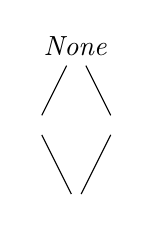
\begin{tikzpicture}
        \node (one) at (0, 0) {\ob};
        \node (conj) at (-0.5, 1) {\cb};
        \node (disj) at (0.5, 1) {\dbb};
        \node (none) at (0, 2) {\textit{None}};
        \draw (one) -- (conj) -- (none) -- (disj) -- (one);
    \end{tikzpicture}
\end{center}

Dove \ob è il minimo e \textit{None} è il massimo.
Il risultato è un reticolo e la funzione compare restituisce l'estremo superiore dei due frammenti.
La funzione complementary restituisce il frammento della negazione di una formula di un determinato frammento.
In particolare il complementare di un \ob è \ob mentre il complementare di un \cb è \dbb e viceversa.



\begin{algorithm}[H] \label{alg:innerClassifier}
    \caption{Classificatore interno}
    \KwSty{Firma:}{ innerClassify($\varphi$)}
    \KwIn{$\varphi$ Una formula rettificata}
    \KwOut{Una coppia (Fragment, Literal)}


\Switch{$\varphi$}{
    \Case{$Literal \; l$}{
        \Return $(ONE\_BINDING, l)$\;
    }
    \Case{$A [\land, \lor] B$}{
        \Return $innerCompare(innerClassify(A), innerClassify(B), \text{connective of } \varphi)$\;
    }
    \Case{$\lnot A$}{
        \Return $innerClassify(A).complementary()$\;
    }
    \Case{$A [\rightarrow, \leftrightarrow, \oplus] B$}{
        \Return $innerCompare(innerClassify(A), innerClassify(B), \text{connective of } \varphi)$\;
    }
    \Else{
        \Return $(None, null)$\;
    }
    
}
\end{algorithm}

La struttura del classificatore interno è molto simile a quella del classificatore esterno, mentre il comparatore interno
è leggermente più complesso. Il caso base è quando la formula è un singolo letterale che è sempre un \ob.
La visita in postOrder restituisce una coppia (Fragment, Literal) che rappresenta il frammento a cui appartiene la formula e un letterale
di rappresentanza della formula in questo caso il letterale più a sinistra. 
Il letterale serve a mantenere una reference alla lista di termini delle formule del frammento \ob.

\begin{algorithm}[H] \label{alg:innerCompare}
    \caption{Compare interno}
    \KwSty{Firma:}{ innerCompare($A, B, con$)}
    \KwIn{$A, B$ due coppie (Fragment, Literal), $con$ un connettivo}
    \KwOut{Una coppia (Fragment, Literal)}



    \Switch{A.first, B.first, con}{
        \Case{One\_Binding, One\_Binding, \_\_}{
            \If{$A.second$ has same terms of $B.second$}{
                \Return $A$\;
            } \ElseIf{$conn = \land$}{
                \Return $(Conjunctive\_Binding, null)$\;
            } \ElseIf{$conn = \lor$}{
                \Return $(Disjunctive\_Binding, null)$\; 
            }
        }

        \Case{[One\_Binding, Conjunctive\_Binding $\mid$ Conjunctive\_Binding, One\_Binding], $\land$}{
            \Return (Conjunctive\_Binding, null)\;
        }
        \Case{[One\_Binding, Disjunctive\_Binding $\mid$ Disjunctive\_Binding, One\_Binding], $\lor$}{
            \Return (Disjunctive\_Binding, null)\;
        }

        \Case{Conjunctive\_Binding, Conjunctive\_Binding, $\land$}{
            \Return (Conjunctive\_Binding, null)\;
        }
        \Case{Disjunctive\_Binding, Disjunctive\_Binding, $\lor$}{
            \Return (Disjunctive\_Binding, null)\;
        }
    }

    \Return $(None, null)$\;
\end{algorithm}


La combinazione booleana di due frammenti \ob (all'interno di un quantificatore) può portare 
a tre diversi risultati.
Se i termini dei letterali di rappresentanza sono uguali allora la combinazione è ancora un \ob altrimenti 
la combinazione è un \cb se il connettivo è $\land$ e un \dbb se il connettivo è $\lor$. 
Il termine \textit{null} viene usato come sostituto del letterale di rappresentanza in formule del frammento \cb e \dbb in quanto 
sono una combinazione di più \ob e non hanno un letterale di rappresentanza.
Due frammenti \cb rimangono \cb solo se il loro connettivo è $\land$.
La combinazione di un \ob con un \cb è un \cb se il connettivo è $\land$. Stesso discorso per i \dbb e il connettivo $\lor$.
In tutti gli altri casi la combinazione è \textit{None}. 
Nell'algoritmo \ref{alg:innerCompare} sono stati omessi i casi con connettivi $\rightarrow, \leftrightarrow, \oplus$ 
in quanto non sono riconducibili a formule composte da $\land$ e $\lor$ come è stato fatto ad esempio nell'algoritmo \ref{alg:classifier}.
Con la funzione complementary applicata ad una coppia: (Fragment, Literal).complementary() si intende la coppia (Fragment.complementary(), Literal).




\end{document}

